\chapter{Ejemplos}
\label{cap:ejemplos}

\section{Ambientes y etiquetas}
\label{sec:etiquetas}

Todos los ambientes que se desee referir por n\'umero m\'as adelante deben de
tener una etiqueta.  Consideremos por ejemplo el siguiente lema.

\begin{lema}
\label{lem:primero}
Primer lema de ejemplo.
\end{lema}

Seguido de un segundo lema.

\begin{lema}
\label{lem:segundo}
Segundo lema de ejemplo.
\end{lema}

Que se utilizan para demostrar \cref{teo:ejemplo}.

\begin{teorema}
\label{teo:ejemplo}
Primer teorema de ejemplo.
\end{teorema}

\begin{proof}
Se sigue de \cref{lem:primero,lem:segundo}.
\end{proof}

Y finalmente obtener el siguiente corolario.

\begin{corolario}
\label{cor:ejemplo}
Corolario de ejemplo.
\end{corolario}

Usando el paquete \href{http://tug.ctan.org/tex-archive/macros/latex/contrib/%
cleveref/cleveref.pdf}{\ttt{cleveref}}\index{cleveref} es posible referirse de
forma sencilla a \cref{lem:primero,lem:segundo,teo:ejemplo,cor:ejemplo} (ver el
c\'odigo correspondiente en \cref{fig:cref}, notando que se utiliz\'o el comando
\ttt{\textbackslash{cref}}).   Este paquete agrega de forma autom\'atica el
nombre del ambiente, e.g., ``el Teorema'', al n\'umero cuando se hace una
referencia.   Esto resulta bastante \'util cuando, por ejemplo, se decide que un
resultado que inicialmente se enunci\'o como un teorema, realmente deber\'ia de
ser un lema; no es necesario buscar todos los lugares donde la referencia
correspondiente ocurre y cambiar los nombres, pues \ttt{cleveref} se encarga de
hacer los cambios.

\begin{figure}[H]
  \centering
  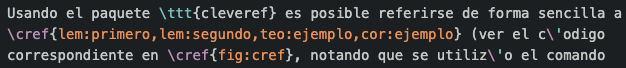
\includegraphics[width=0.8\textwidth]{recursos/capturas/cref}
  \caption{Ejemplo de uso de \ttt{\textbackslash{cref}}.}
  \label{fig:cref}
\end{figure}

Sin embargo, la gram\'atica del espa\~nol hace necesario introducir variantes en
algunos casos especiales, como cuando hacemos referencia ``al Teorema
\ref{teo:ejemplo}'' (n\'otese que se utiliz\'o ``al Teorema'' en lugar de ``el
Teorema''), o queremos decir que un resultado es una consecuencia ``del
Corolario \ref{cor:ejemplo}''.   En este caso, necesitamos agregar el nombre del
ambiente a mano, y usar el comando habitual \ttt{\textbackslash{ref}}.   El
autor del presente documento prefiere utilizar siempre may\'usculas cuando se
usa el nombre de un ambiente referido por n\'umero, e.g., ``\cref{teo:ejemplo}''
en lugar de ``el teorema \ref{teo:ejemplo}'', por lo que esta configuraci\'on se
ve reflejada en el archivo \ttt{tesis.tex}, cuando se utiliza el comando
\ttt{\textbackslash{crefname}} para definir los nombres de ambiente que debe de
usar \ttt{cleveref}.

Una alternativa para evitar algunos de los problemas descritos en el p\'arrafo
anterior es definir el nombre del ambiente sin utilizar el art\'iculo, e.g.,
``Teorema'' en lugar de ``el Teorema''.   Aunque esto permite un poco m\'as de
flexibilidad, cuando es necesario cambiar un ambiente con nombre masculino a uno
con nombre femenino, o viceversa (por ejemplo proposici\'on por lema), es
necesario realizar todos los cambios de los art\'iculos a mano.  Adicionalmente,
(y el motivo principal por el que se decidi\'o no usar esta variante) el uso del
paquete como el mostrado en el ejemplo de \cref{fig:cref} dejar\'ia de
funcionar, pues los art\'iculos ser\'ian omitidos, generando una construcci\'on
gramatical incorrecta.

Si no se desea usar el paquete \ttt{cleveref}, siempre puede omitirse y utilizar
\'unicamente el comando \ttt{\textbackslash{ref}} que est\'a incluido por
omisi\'on en \LaTeX.

Adem\'as de los ambientes, tambi\'en es posible etiquetar cap\'itulos o
secciones, y referirnos a la p\'agina donde aparece una etiqueta dada.   Por
ejemplo, podemos referirnos a \cref{sec:dibujos} en la \cpageref{sec:dibujos}, o
al Cap\'itulo \ref{cap:ejemplos}.   La referencia a las p\'aginas es \'util en
la versi\'on impresa del documento, aunque en la versi\'on digital parezca un
poco in\'util gracias a que cada referencia es una liga al objeto en cuesti\'on.



\section{Dibujos y colores}
\label{sec:dibujos}

Los dibujos pueden agregarse de al menos dos formas obvias.   La primera es
hacerlos dentro de \LaTeX con alg\'un paquete como
\href{https://github.com/pgf-tikz/pgf}{\ttt{tikz}}\index{tikz}.   La segunda es
generarlos con alg\'un recurso externo, e incluirlo con el comando
\ttt{\textbackslash{includegraphics}}.   Tambi\'en puede usarse una
combinaci\'on de ambos, generando un PDF con la imagen en un archivo externo de
\LaTeX, y agreg\'andolo con \ttt{\textbackslash{includegraphics}}; una ventaja
de esta tercera posibilidad es que el compilador realiza menos trabajo para
generar el documento.

En \cref{fig:grafica} podemos ver un ejemplo de un dibujo hecho con \ttt{tikz}.
Una ventaja de hacer los dibujos dentro de \LaTeX{} es que resulta f\'acil
agregar f\'ormulas o etiquetas con la misma tipograf\'ia que el resto del
documento.

\begin{figure}[ht!]
\centering
\begin{tikzpicture}
\node (0) [vertex,label=180:$v_1$] at (0,0){};
\node (1) [vertex,label=90:$v_2$]  at (1,0){};
\begin{scope}[xshift=2cm]
\node (2) [vertex,label=90:$v_3$]  at (270:1){};
\node (3) [vertex,label=0:$v_4$]   at (0:1){};
\node (4) [vertex,label=90:$v_5$]  at (90:1){};
\end{scope}

\draw [myloop,in=60,out=120,looseness=12]
      (0) to node[above]{$e_1$} (0);
\draw [myloop,in=240,out=300,looseness=12]
      (0) to node[below]{$e_2$} (0);
\draw [myloop,in=240,out=300,looseness=12]
      (2) to node[below]{$e_9$} (2);

\draw [edge]               (0) to node [above] {$e_3$} (1);
\draw [edge]               (1) to node [below] {$e_4$} (2);
\draw [edge]               (2) to node [below] {$e_5$} (3);
\draw [edge,bend right=20] (3) to node [above] {$e_6$} (4);
\draw [edge,bend left=20]  (3) to node [below] {$e_7$} (4);
\draw [edge]               (4) to node [above] {$e_8$} (1);


% Componente derecha
\begin{scope}[xshift=6cm]
\node (5) [vertex,label=90:$v_6$]    at (0:1.5){};
\node (6) [vertex,label=120:$v_7$]   at (120:1.5){};
\node (7) [vertex,label=240:$v_8$]   at (240:1.5){};
\node (8) [vertex,label=0:$v_9$]     at (3,1.2){};
\node (9) [vertex,label=0:$v_{10}$]  at (3,-1.2){};

\draw [edge,bend right=10] (5) to node [above] {$e_{10}$} (6);
\draw [edge,bend left=10]  (5) to node [below] {$e_{11}$} (6);
\draw [edge,bend right=10] (6) to node [left]  {$e_{12}$} (7);
\draw [edge,bend left=10]  (6) to node [right] {$e_{13}$} (7);
\draw [edge,bend right=10] (7) to node [below] {$e_{14}$} (5);
\draw [edge,bend left=10]  (7) to node [above] {$e_{15}$} (5);
\draw [edge]               (5) to node [above] {$e_{16}$} (8);
\draw [edge]               (5) to node [below] {$e_{17}$} (9);
\end{scope}

\end{tikzpicture}
\caption{El diagrama de una gr\'afica con lazos y
aristas m\'ultiples.}
\label{fig:grafica}
\end{figure}

Es f\'acil agregar colores a los dibujos.   Hay que tener presente que
\ttt{tikz} construye el dibujo por capas, y el c\'odigo se ejecuta de forma
secuencial, por lo que la \'ultima parte del c\'odigo es la \'ultima capa que se
dibujar\'a, y puede cubrir a otras, generando un resultado distinto al deseado.
Es posible definir colores nuevos mediante el comando
\ttt{\textbackslash{definecolor}}, en el caso de este documento, todos los
colores nuevos se definen en el archivo \ttt{tesis.tex}.   Las diferentes
opciones para el comando \ttt{\textbackslash{definecolor}} se encuentran
explicadas \href{https://en.wikibooks.org/wiki/LaTeX/Colors}{aqu\'i}.

Para agregar colores en el texto, o en las celdas de una tabla, u otros lugares,
se puede utilizar el paquete
\href{https://ctan.org/pkg/xcolor}{\ttt{xcolor}}\index{xcolor}.  Una forma
sencilla de usar color en el texto es con la construcci\'on
\begin{lstlisting}
{\color{nombre-del-color}texto con color}}
\end{lstlisting}
{\color{verdeAzulado}lo que permite generar texto de color.

Incluso es posible usar un color a lo largo de distintos p\'arrafos.}


\begin{figure}[ht!]
\begin{tikzpicture}
%%%%%%%%%%%%%%%%%%%%%%%%%%%%%%%%%%%%%%%%%%%%%%%%
%%%%%%%%%%         Empty Graph        %%%%%%%%%%
%%%%%%%%%%%%%%%%%%%%%%%%%%%%%%%%%%%%%%%%%%%%%%%%
\begin{scope}
% if label is needed -> label={(360/4)*\i}:$\i$
\foreach \i in {0,...,3}
	\node (\i) [vertex,fill=cyan] at ({(360/4)*\i}:1){};

\node (L) at (-1,1){$G_1$};
\end{scope}

%%%%%%%%%%%%%%%%%%%%%%%%%%%%%%%%%%%%%%%%%%%%%%%%
%%%%%%%%%%       Complete Graph       %%%%%%%%%%
%%%%%%%%%%%%%%%%%%%%%%%%%%%%%%%%%%%%%%%%%%%%%%%%
\begin{scope}[xshift=3.1cm,yshift=-0.3cm]
\node (4) [vertex,fill=verdeAzulado] at (0,0){};
\foreach \i in {0,1,2}
	\node (\i) [vertex,fill=verdeAzulado] at ({90+(360/3)*\i}:1.2){};

\foreach \i in {0,1,2}
	\draw [edge] let \n1={int(mod(\i+1,3))} in (\i) to (\n1);
\foreach \i in {0,1,2}
	\draw [edge] (\i) to (4);

\node (L) at (-1,1){$G_2$};
\end{scope}


%%%%%%%%%%%%%%%%%%%%%%%%%%%%%%%%%%%%%%%%%%%%%%%%
%%%%%%%%%%       Bipartite Graph      %%%%%%%%%%
%%%%%%%%%%%%%%%%%%%%%%%%%%%%%%%%%%%%%%%%%%%%%%%%
\begin{scope}[xshift=6.2cm,yshift=0cm]
\foreach \i in {0,2,4}
	\node (\i) [vertex,fill=red]  at ({(360/6)*\i}:1){};
\foreach \i in {1,3,5}
	\node (\i) [vertex,fill=blue] at ({(360/6)*\i}:1){};

\foreach \i in {0,...,5}
	\draw [edge] let \n1={int(mod(\i+1,6))} in (\i) to (\n1);

\node (L) at (-1,1){$G_3$};
\end{scope}


%%%%%%%%%%%%%%%%%%%%%%%%%%%%%%%%%%%%%%%%%%%%%%%%
%%%%%%%%%%            Star            %%%%%%%%%%
%%%%%%%%%%%%%%%%%%%%%%%%%%%%%%%%%%%%%%%%%%%%%%%%
\begin{scope}[xshift=9.3cm]
\node (6) [vertex,fill=violet] at (0,0){};
\foreach \i in {0,...,4}
	\node (\i) [vertex,fill=green] at ({90+(360/5)*\i}:1){};

\foreach \i in {0,...,4}
	\draw [edge] (\i) to (6);

\node (L) at (-1,1){$G_4$};
\end{scope}


%%%%%%%%%%%%%%%%%%%%%%%%%%%%%%%%%%%%%%%%%%%%%%%%
%%%%%%%%%%           Split            %%%%%%%%%%
%%%%%%%%%%%%%%%%%%%%%%%%%%%%%%%%%%%%%%%%%%%%%%%%
\begin{scope}[xshift=12.4cm]
\foreach \i in {0,2,4}
	\node (\i) [vertex,fill=black] at ({30+(360/6)*\i}:0.7){};
\foreach \i in {1,3,5}
	\node (\i) [vertex] at ({30+(360/6)*\i}:1.4){};

\foreach \i in {0,...,5}
	\draw [edge] let \n1={int(mod(\i+1,6))} in (\i) to (\n1);
\foreach \i in {0,2,4}
	\draw [edge] let \n1={int(mod(\i+2,6))} in (\i) to (\n1);

\node (L) at (-1,1){$G_5$};
\end{scope}

\end{tikzpicture}
\caption{Ejemplos de gr\'aficas vac\'ia, completa,
bipartita, bipartita completa y escindible.}
\label{fig:fam1}
\end{figure}

Continuando con los dibujos, resulta bastante \'util usar ciclos \ttt{for}
dentro de \ttt{tikz} para realizar dibujos que tienen simetr\'ias.   Un ejemplo
de esto ocurre en \cref{fig:fam1}.   En \cref{fig:tikzFor}, se observa el
c\'odigo del ciclo azul y rojo que aparece en \cref{fig:fam1}.

\begin{figure}[ht!]
  \centering
  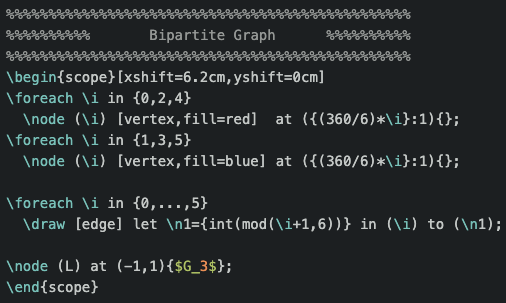
\includegraphics[width=0.8\textwidth]{recursos/capturas/tikzfor}
  \caption{Ejemplo de un ciclo \ttt{for} dentro de \ttt{tikz}.}
  \label{fig:tikzFor}
\end{figure}

Aunque en este caso los ejemplos se concentran en dibujar gr\'aficas, las
posibilidades de \ttt{tikz} son gigantescas.   Se recomienda al usuario revisar
el \href{https://mirror.las.iastate.edu/tex-archive/graphics/pgf/base/doc/%
pgfmanual.pdf}{manual de PGF y TikZ}.


\section{Algoritmos}

Para los algoritmos utilizamos el paquete \href{https://www.ctan.org/pkg/%
algorithm2e}{\ttt{algorithm2e}}\index{algorithm2e}.   En este caso simplemente
se presentar\'a un ejemplo de uso con un subconjunto limitado de las distintas
opciones que se pueden utilizar.   Se recomienda revisar la documentaci\'on del
paquete para conocer todas las posibilidades.

\begin{algorithm}[ht!]
\SetAlgorithmName{Algoritmo}{}
  \DontPrintSemicolon
  \SetKwData{False}{false}\SetKwData{True}{true}
  \SetKwFunction{New}{new}\SetKwFunction{End}{end}\SetKwFunction{Used}{used}
  \SetKwInOut{Input}{input}\SetKwInOut{Output}{output}

  \KwIn{Una gr\'afica conexa $G$ con un v\'ertice distingido $r$.}
  \KwOut{Funciones de parentesco $p$, nivel $\ell$ y tiempo de exploraci\'on
         $t$.}
  \BlankLine
  $Q \leftarrow []$; $i \leftarrow 0$\;
  $i \leftarrow i+1$\;
  colorear a $r$ de negro\;
  a\~nadir $r$ al final de $Q$\;
  $t(r) \leftarrow i$, $p(r) \leftarrow \varnothing$, $\ell (r) \leftarrow 0$\;
  {\While{$Q \ne []$}{
  	elegir a la cabeza $x$ de $Q$\;
 	\If{$x$ tiene un vecino $y$ sin colorear}{
		$i \leftarrow i+1$\;
		colorear a $y$ de negro\;
		a\~nadir $y$ al final de $Q$\;
		$t(y) \leftarrow i$, $p(y) \leftarrow x$, $\ell(y) \leftarrow \ell(x) + 1$\;
	}\Else{
		eliminar $x$ de $Q$\;
	}
  }
  }
  {\Return $(p,\ell,t)$}
  \caption{Breadth First Search}
  \label{alg:bfs}
\DecMargin{1em}
\end{algorithm}

\Cref{alg:bfs} muestra algunas opciones sencillas del paquete.   Quiz\'a la
observaci\'on m\'as importante para considerar respecto a \ttt{algorithm2e} es
que, por dise\~no, el paquete no divide los algoritmos para aparecer en m\'as
de una p\'agina.   Por lo tanto, un algoritmo largo usualmente se recorrer\'a
a la siguiente p\'agina (y posiblemente ocupar\'a una p\'agina completa).

\section{\'Indice alfab\'etico}
\label{sec:indice}

Es posible agregar palabras al \'indice\index{indice@\'indice} alfab\'etico
usando el comando \ttt{\textbackslash{index}}.   Un uso t\'ipico es el
siguiente; supongamos que se desea agregar la palabra ``gr\'afica'' al \'indice,
entonces es necesario escribir la palabra, seguida de la misma palabra dentro
del comando.
\begin{lstlisting}
gr\'afica\index{gr\'afica}
\end{lstlisting}

Cuando se introduce un concepto nuevo, es deseable resaltarlo de alguna forma en
el texto.   En los art\'iculos usualmente se utilizan \textit{cursivas} y en los
libros (o una tesis), generalmente se prefieren las \textbf{negritas}.   Por
este motivo, se agreg\'o al pre\'ambulo un comando para poner, al mismo tiempo,
una palabra en negritas y agregarla al \'indice; el comando es
\ttt{\textbackslash{indice}}.   Por ejemplo, dicho comando est\'a siendo
utilizado en la palabra \indice{concepto}, mismo que se puede verificar aparece
en el \'indice anal\'itico al final del documento. Tambi\'en es com\'un
encontrar una versi\'on especializada de un concepto, e.g., la definici\'on de
gr\'afica bipartita depende de la de gr\'afica.   En este sentido, es deseable
que ``gr\'afica bipartita'' aparezca como una entrada que depende de
``gr\'afica''.   Para lograr esto se utiliza el mismo comando
\ttt{\textbackslash{index}}, con la siguiente sintaxis.
\begin{lstlisting}
\index{concepto!subconcepto}
\end{lstlisting}

De manera an\'aloga al caso del comando \ttt{\textbackslash{indice}}, se cre\'o
un comando \ttt{\textbackslash{indiceSub}}, que toma dos argumentos.  El primero
es la entrada principal que aparecer\'a en el \'indice (e.g., gr\'afica), y la
segunda es la versi\'on especializada que depende de la primera (e.g.,
bipartita).   Para brindar libertad en la forma de redactar las definiciones,
\ttt{\textbackslash{indiceSub}} s\'olo imprime en el documento el segundo
argumento.   Por ejemplo, en \indiceSub{concepto}{subconcepto} se utiliz\'o
\ttt{\textbackslash{indiceSub}} con los argumentos \ttt{concepto} y
\ttt{subconcepto} (puede verificarse el funcionamiento en el \'indice).

Dependiendo del editor que se est\'e utilizando para trabajar con \LaTeX, es
posible que el \'indice no se actualice autom\'aticamente.   De ser el caso,
basta con ejecutar el siguiente comando en el directorio del proyecto donde se
encuentre el archivo \ttt{tesis.idx} (\'este \'ultimo se genera
autom\'aticamente al compilar \ttt{tesis.tex}).
\lstset{language=bash}
\begin{lstlisting}
makeindex tesis.idx
\end{lstlisting}

El comando anterior generar\'a el archivo \ttt{tesis.ind}, mismo que contiene la
informaci\'on necesaria para incluir el \'indice en el PDF final.

Los conceptos aparecen en orden alfab\'etico en el \'indice, sin embargo, el uso
de caracteres especiales (como letras acentuadas) afecta el orden habitual.
Para corregir problemas derivados del uso de caracteres especiales, se refiere
al lector al siguiente \href{https://en.wikibooks.org/wiki/LaTeX/%
Indexing#Using_special_characters}{art\'iculo sobre indexaci\'on}.
